\chapter{构建与代码分析环境}
\label{ch:env}
\section{编译}


编译hadoop非常简单,首先需要安装Apache Ant,Ant是一个将JAVA软件编译、测试、部署等步骤集成起来的自动化工具,在安装好Ant之后,在common、hdfs、mapreduce目录下分别执行``ant jar''命令,ant系统会自动地根据build.xml和build target,自动下载所需的依赖。

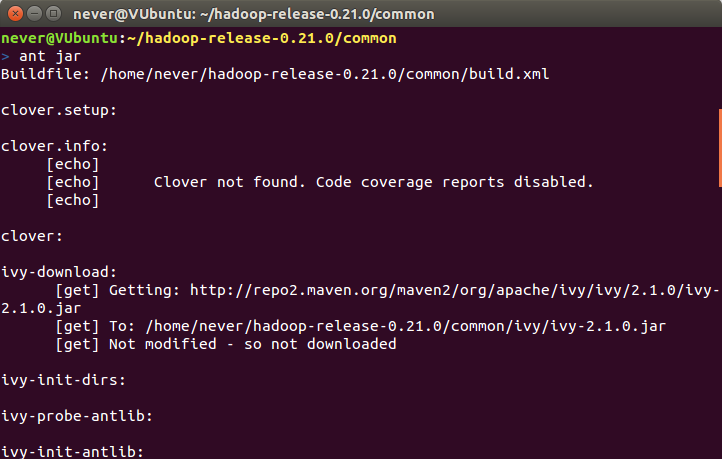
\includegraphics[width=\textwidth]{image/env/cr0.png}

编译成功

![](cr0.1.png)

同理,在hdfs、mapreduce中执行相同的命令即可


\section{配置}

本节介绍Hadoop文件系统的基本配置,包括使用HDFS和使用本地文件系统的例子。
由于环境条件的限制,加之本文的重点在于对Hadoop文件系统架构的分析,
在此,针对HDFS,我们只在本机上配置一个单namenode,单datanode
的伪集群环境,但是相关操作都仿照集群操作进行。

为了本节配置说明的普遍性,没有使用上面手动编译的版本,而是使用了已经编译好的版本来进行配置,
手动编译的版本配置与此类似。

\section{SSH}

首先,为了能够自动地启动所有的node,我们需要在集群机器间配置SSH
服务,这样就可以通过脚本来远程启动node上指定的服务。

首先要在集群的各台电脑上安装ssh服务

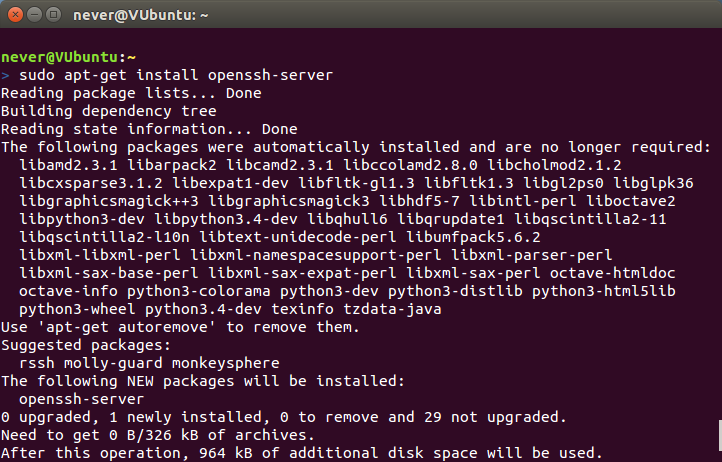
\includegraphics[width=\textwidth]{image/env/cr1.png}

生成密匙对

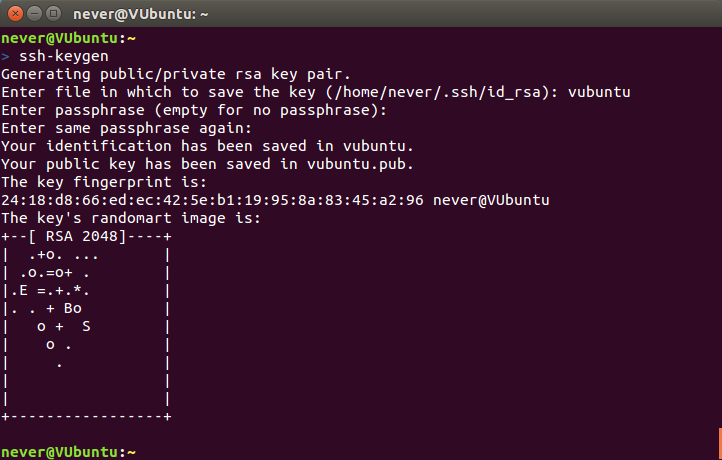
\includegraphics[width=\textwidth]{image/env/cr2.png}

将密匙对拷贝到集群各节点的用户目录下的.ssh文件夹

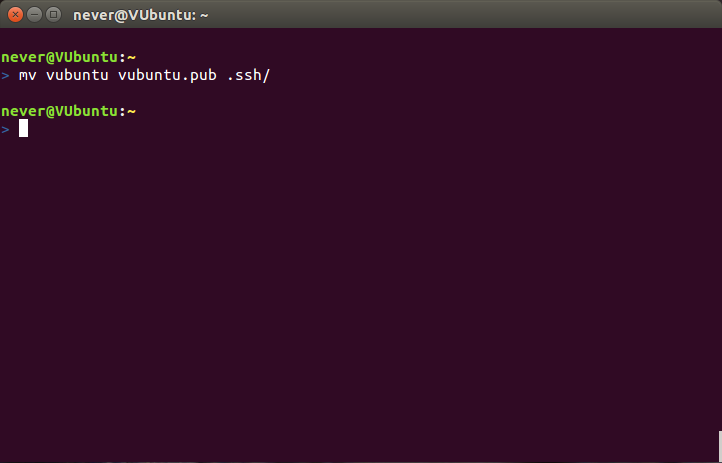
\includegraphics[width=\textwidth]{image/env/cr3.png}

验证是否可以使用ssh命令免密码登录

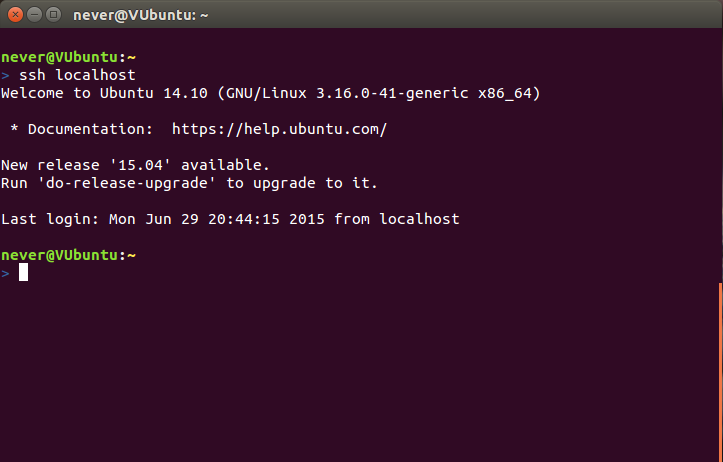
\includegraphics[width=\textwidth]{image/env/cr4.png}

成功之后进入下一步

\section{JAVA环境配置}

在这里我们需要设置三个环境变量,分别是{\JH},{\CPATH},{\HHOME}

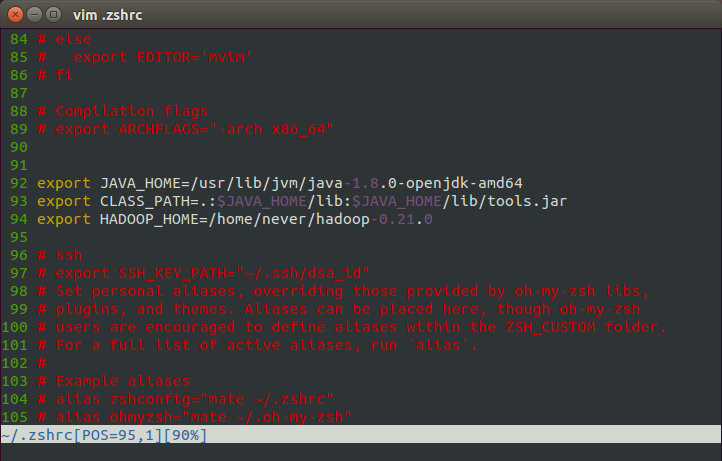
\includegraphics[width=\textwidth]{image/env/cr5.png}

{\JH}和{\CPATH}按照基本的Java环境配置即可,{\HHOME}指向的是
我们将hadoop0.21版本的文件解压到的位置,里面目录结构如下

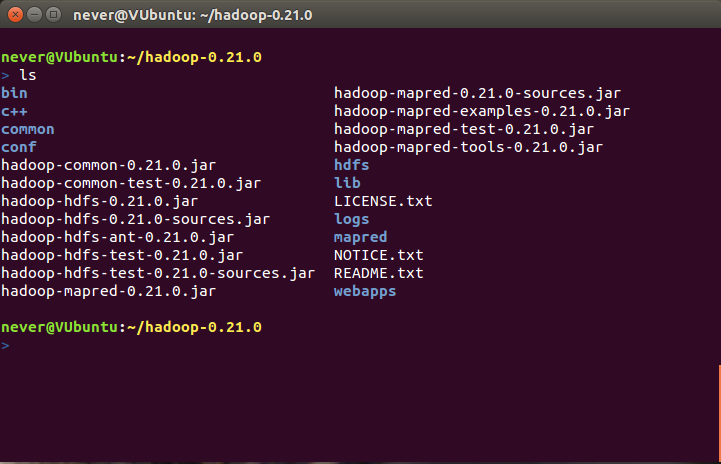
\includegraphics[width=\textwidth]{image/env/cr6.png}

\section{Hadoop配置}

首先是对于本地文件系统,Hadoop不需要进行配置,使用默认配置,
使用命令即可

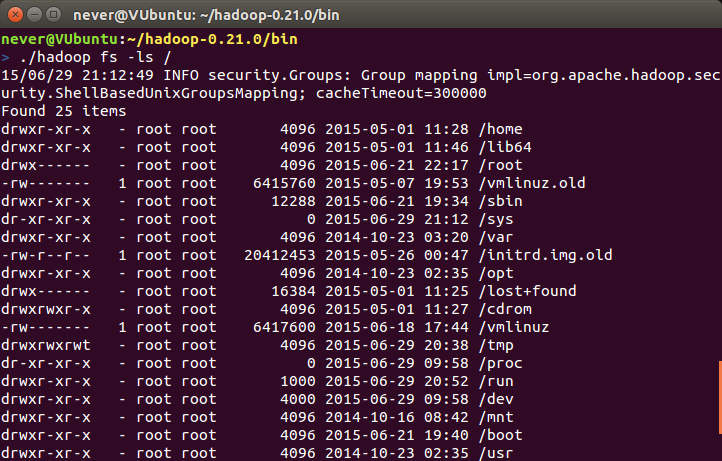
\includegraphics[width=\textwidth]{image/env/cr7.png}

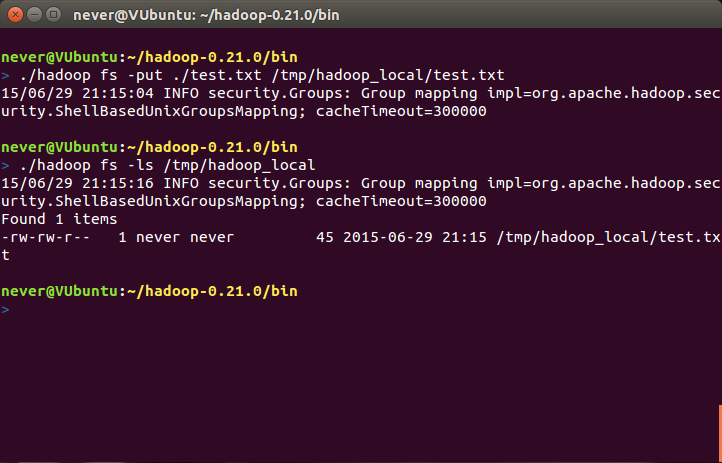
\includegraphics[width=\textwidth]{image/env/cr8.png}

如果使用HDFS作为文件系统,那么需要做如下的配置

首先是conf/core-site.xml,这是设置了hadoop主要的参数

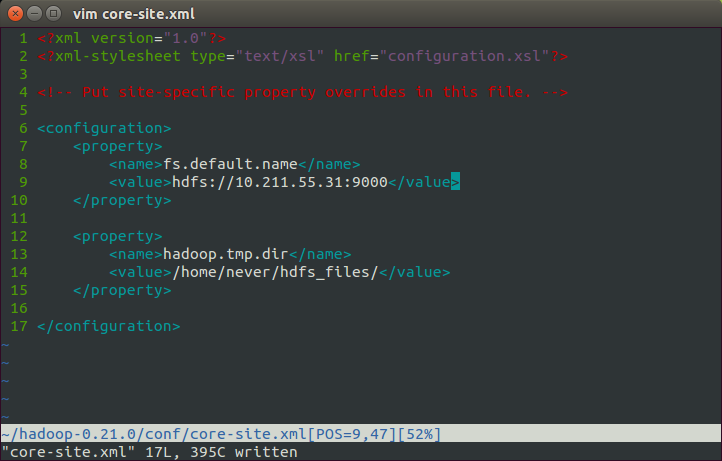
\includegraphics[width=\textwidth]{image/env/cr9.png}

其中fs.default.name选项指定了默认的文件系统,此时指定了默认的文件系统为hdfs,其namenode的ip地址
为10.211.55.31,端口为9000。

hadoop.tmp.dir指定了hdfs中datanode存放文件块的位置。

然后是conf/hdfs-site.xml,这里设置了HDFS的相关参数

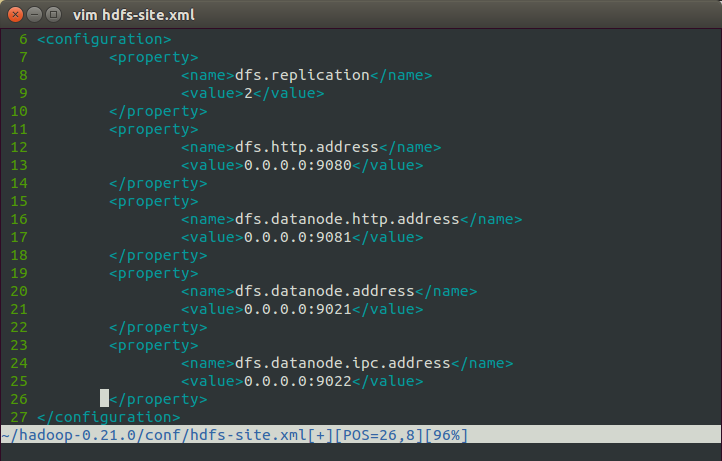
\includegraphics[width=\textwidth]{image/env/cr10.png}

其中dfs.replication指定了文件block副本的数量

dfs.http.address指定了namenode的http服务端口,可以使用浏览器访问这个端口,来
观察整个系统的运行情况,效果如下

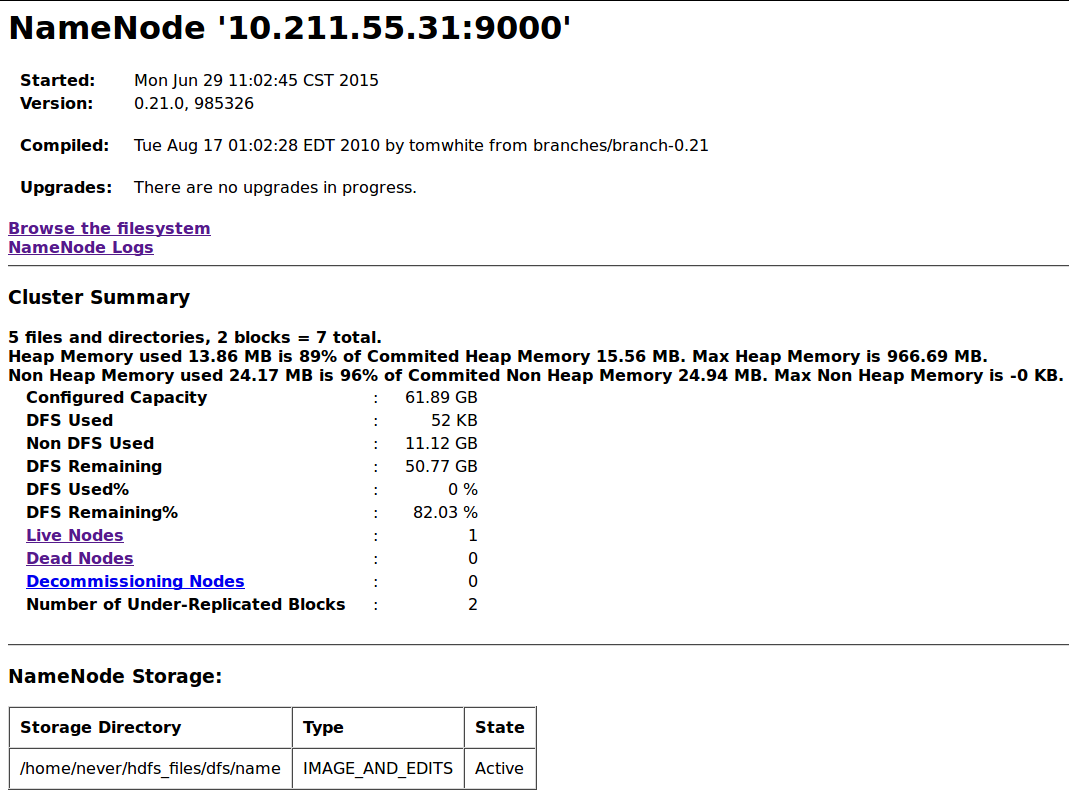
\includegraphics[width=\textwidth]{image/env/cr11.png}

dfs.datanode.http.address指定了datanode的http服务端口,可以使用浏览器访问这个端口,来
观察整对应的datanode的运行情况,效果如下

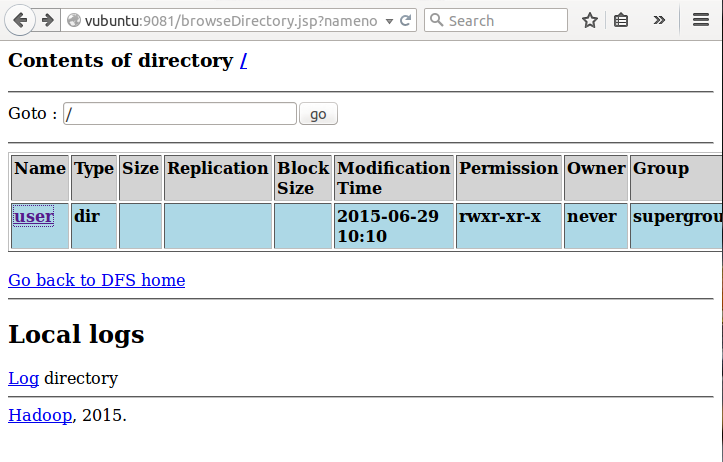
\includegraphics[width=\textwidth]{image/env/cr12.png}

dfs.datanode.address,指定了datanode服务的监听端口

dfs.datanode.ipc.address,指定了datanode的ipc服务监听端口

接下来是master何slave节点的配置,分别对应namenode和datanode

conf/master

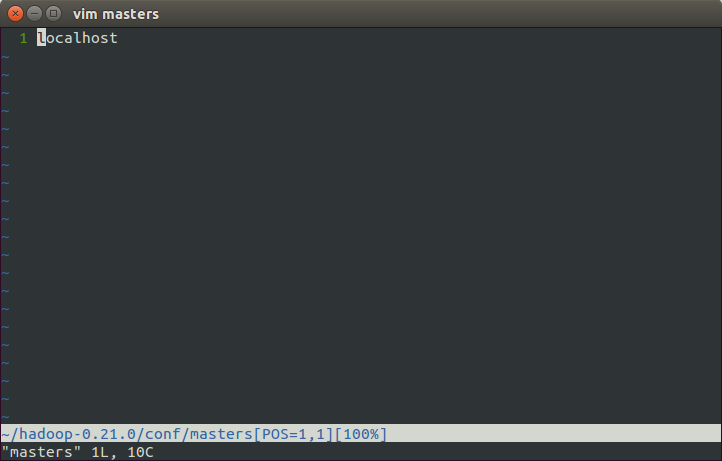
\includegraphics[width=\textwidth]{image/env/cr13.png}

conf/slaves

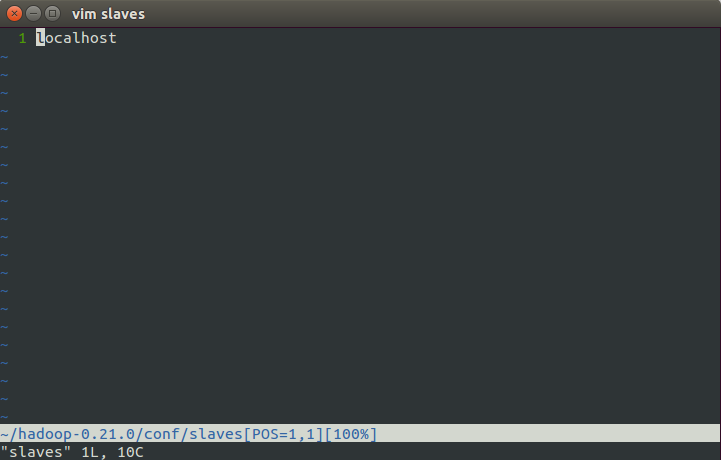
\includegraphics[width=\textwidth]{image/env/cr14.png}

接下来执行bin/start-all.sh来启动namenode和datanode,这一步同样会在namenode上启动job tracker来
准备执行MapReduce任务

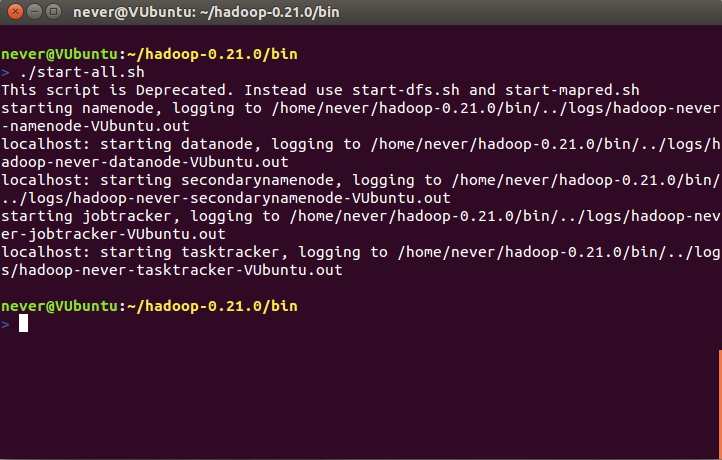
\includegraphics[width=\textwidth]{image/env/cr15.png}

然后可以执行如下的命令来观察启动成功后的效果

\section{运行过程分析}

现在我们来对Hadoop文件系统的运行过程进行分析

从Hadoop命令的执行脚本开始,bin/hadoop

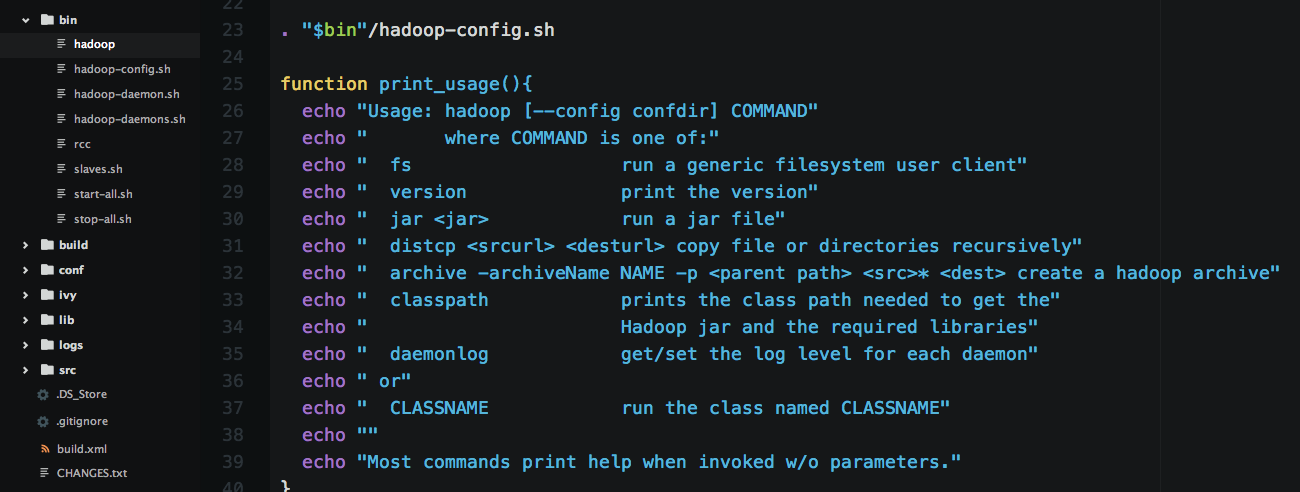
\includegraphics[width=\textwidth]{image/env/cr16.png}

可以看到,如果执行命令的第二个参数是``dfs'',那么则会执行如下的语句,可以这里会调用另外一个脚本hdfs/bin/hdfs

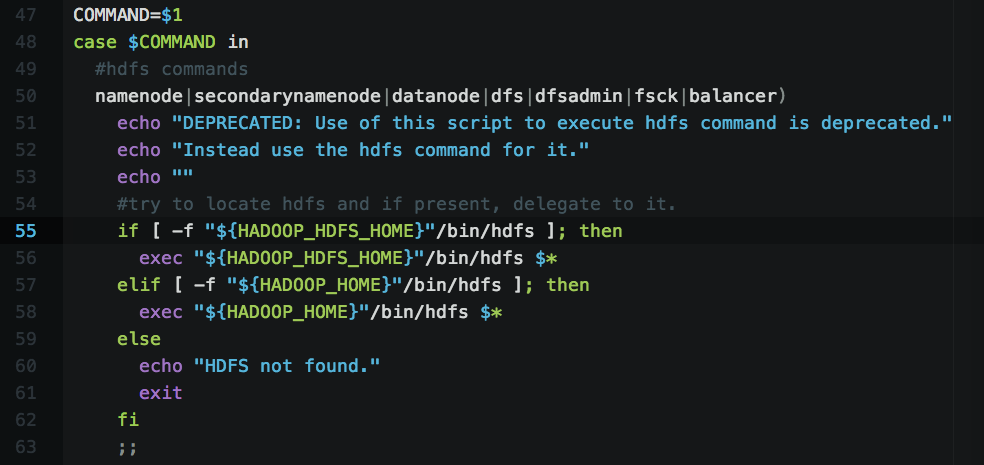
\includegraphics[width=\textwidth]{image/env/cr17.png}

hdfs脚本如下所示

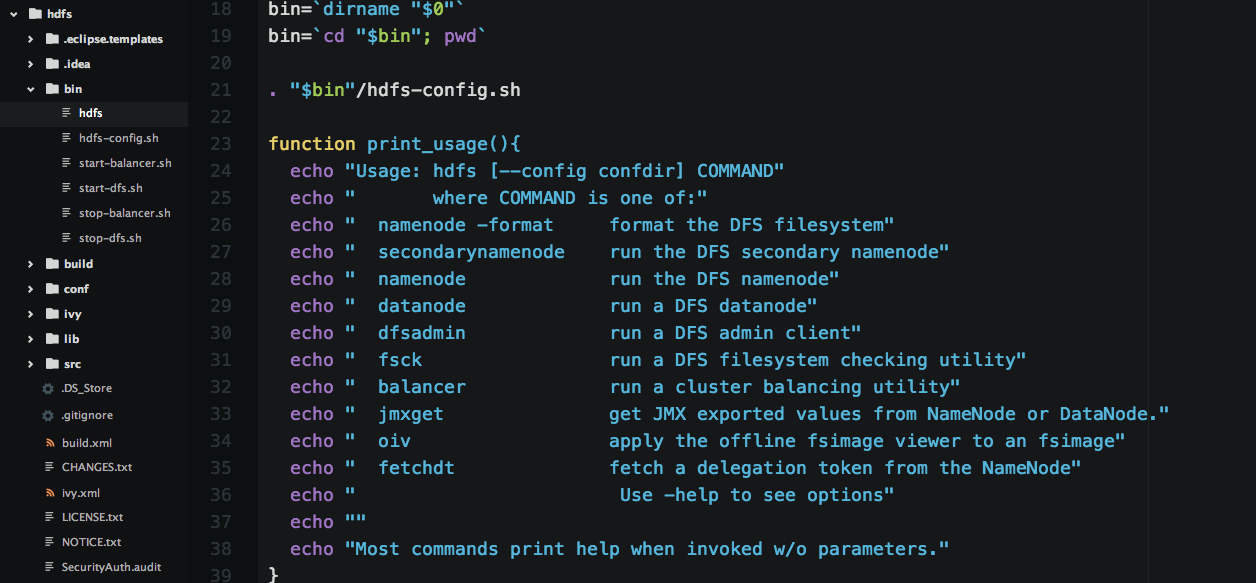
\includegraphics[width=\textwidth]{image/env/cr18.png}

可以看到hdfs脚本最后会调用java命令,并添加相关的虚拟机选项,指定{\CPATH},如果仔细观察,在bin/hadoop这个脚本中,在最后也有类似的命令,如果第二个参数指定为``fs'',那么则会执行bin/hadoop尾部的命令,而在此处然后最后执行main所在的目标类是org.apache.hadoop.fs.FsShell

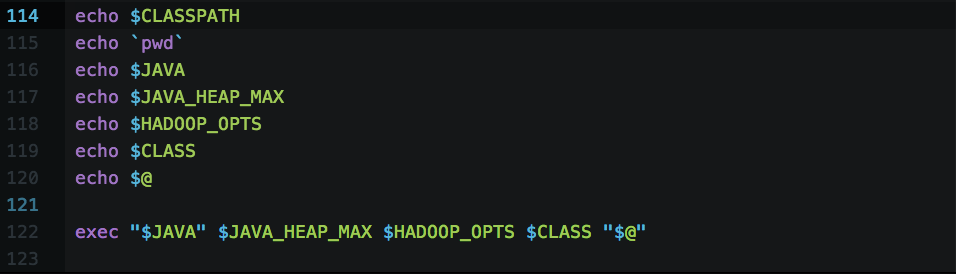
\includegraphics[width=\textwidth]{image/env/cr19.png}

在加上调试参数之后,执行如下命令

	 ./hadoop dfs -ls

运行结果如下

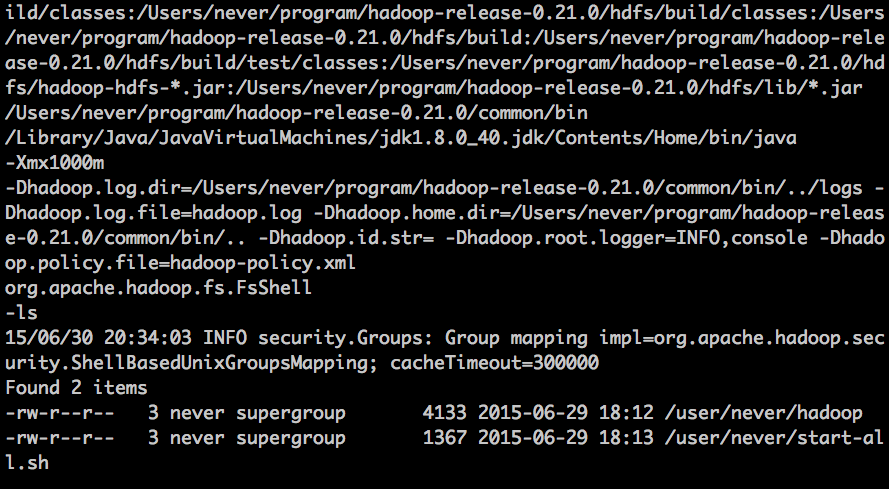
\includegraphics[width=\textwidth]{image/env/cr20.png}

根据上面的观察,可以发现,Hadoop文件系统的运行基于Shell脚本,Shell脚本可以根据执行的命令的不同,设置合适的{\CPATH}等相关参数。

了解了hadoop,运行脚本相关机制,接下来进入IDE的配置,这样便于使用调试器来观察。

我们没有使用Eclipse,而是使用JetBrains的IntelliJ IDEA作为开发环境,主要是因为Eclipse的稳定性欠佳,而且IDEA是一款在各方面都十分优秀的JAVA IDE,所以,我们此次的相关实验内容都在IDEA下完成,使用的IDEA版本是14.1.4,操作系统使用的是MAC OSX 10.10.3。

首先,新建一个空的工程,名为HadoopCommon

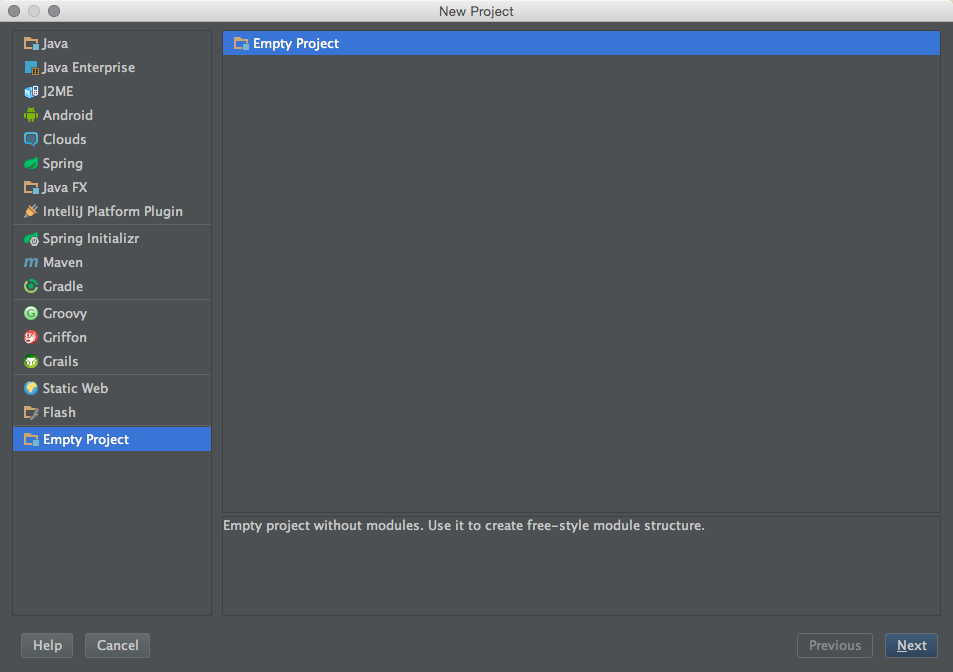
\includegraphics[width=\textwidth]{image/env/cr21.png}

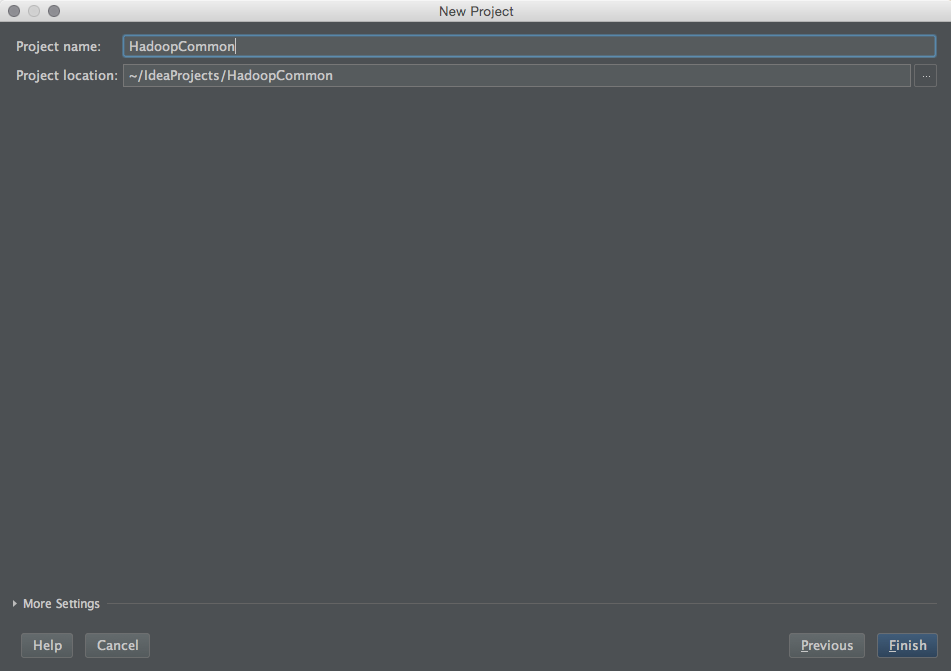
\includegraphics[width=\textwidth]{image/env/cr22.png}

在Project Structure中的Project页面配置使用的JDK为JDK1.6

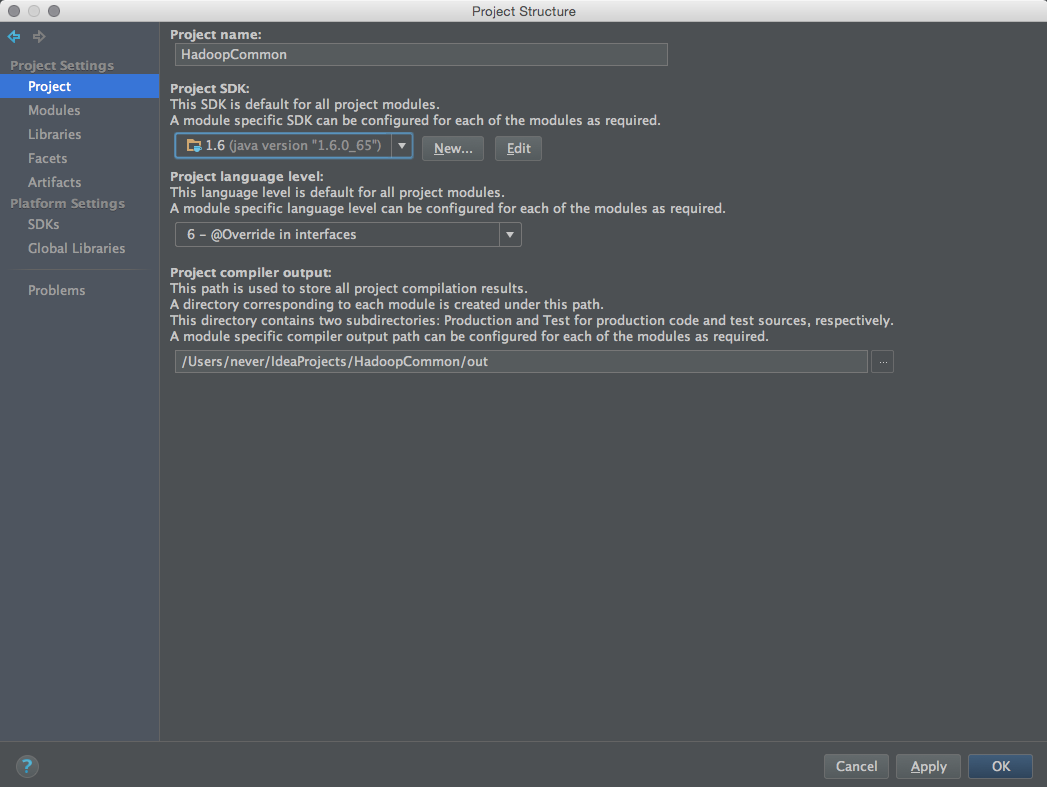
\includegraphics[width=\textwidth]{image/env/cr23.png}

在Modules页面加入一个新的Module,使用默认的JAVA EE7 即可,Module Name为java

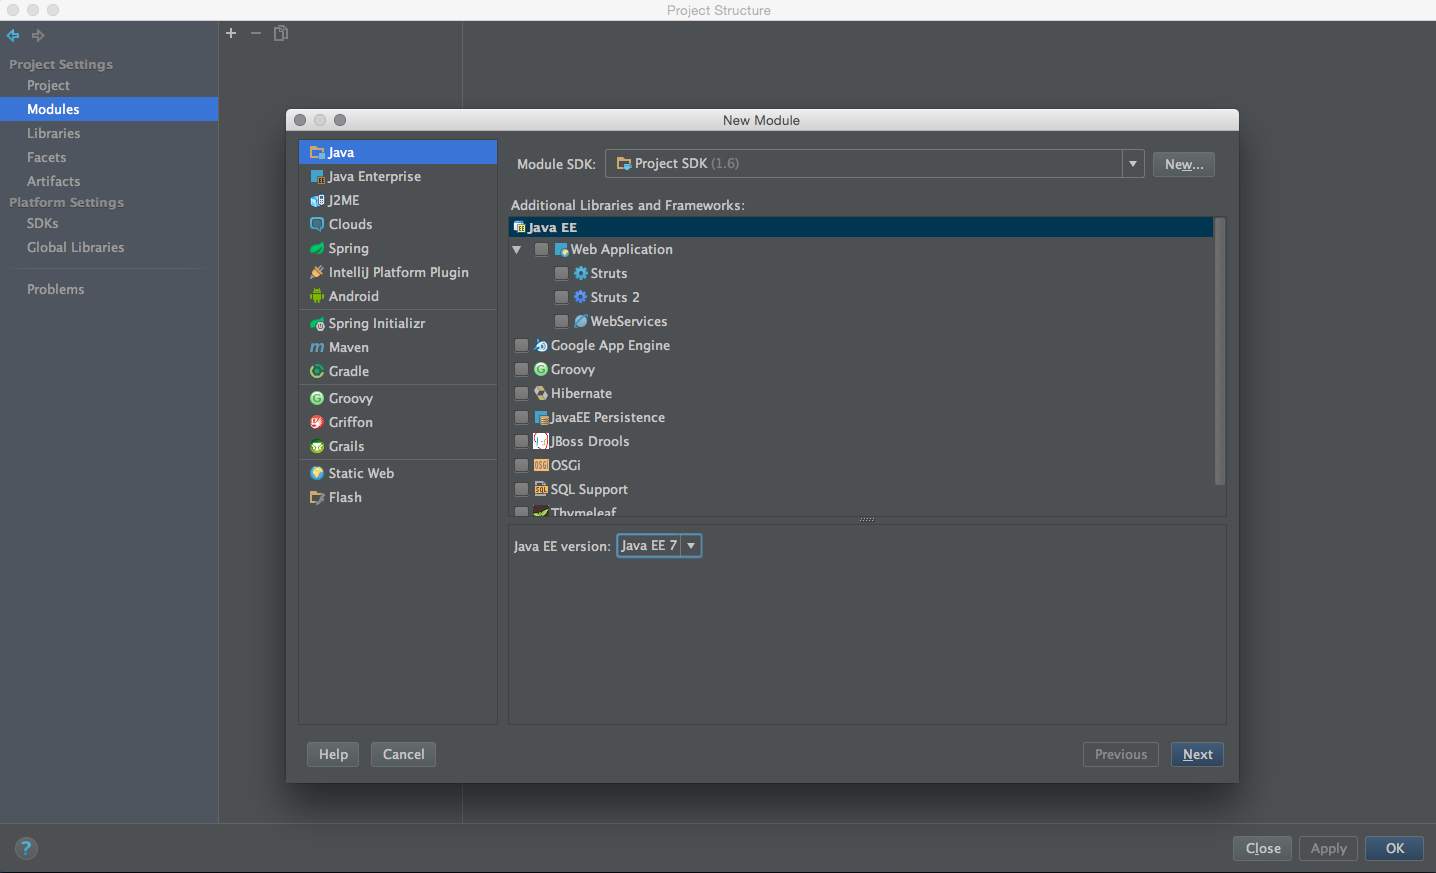
\includegraphics[width=\textwidth]{image/env/cr24.png}

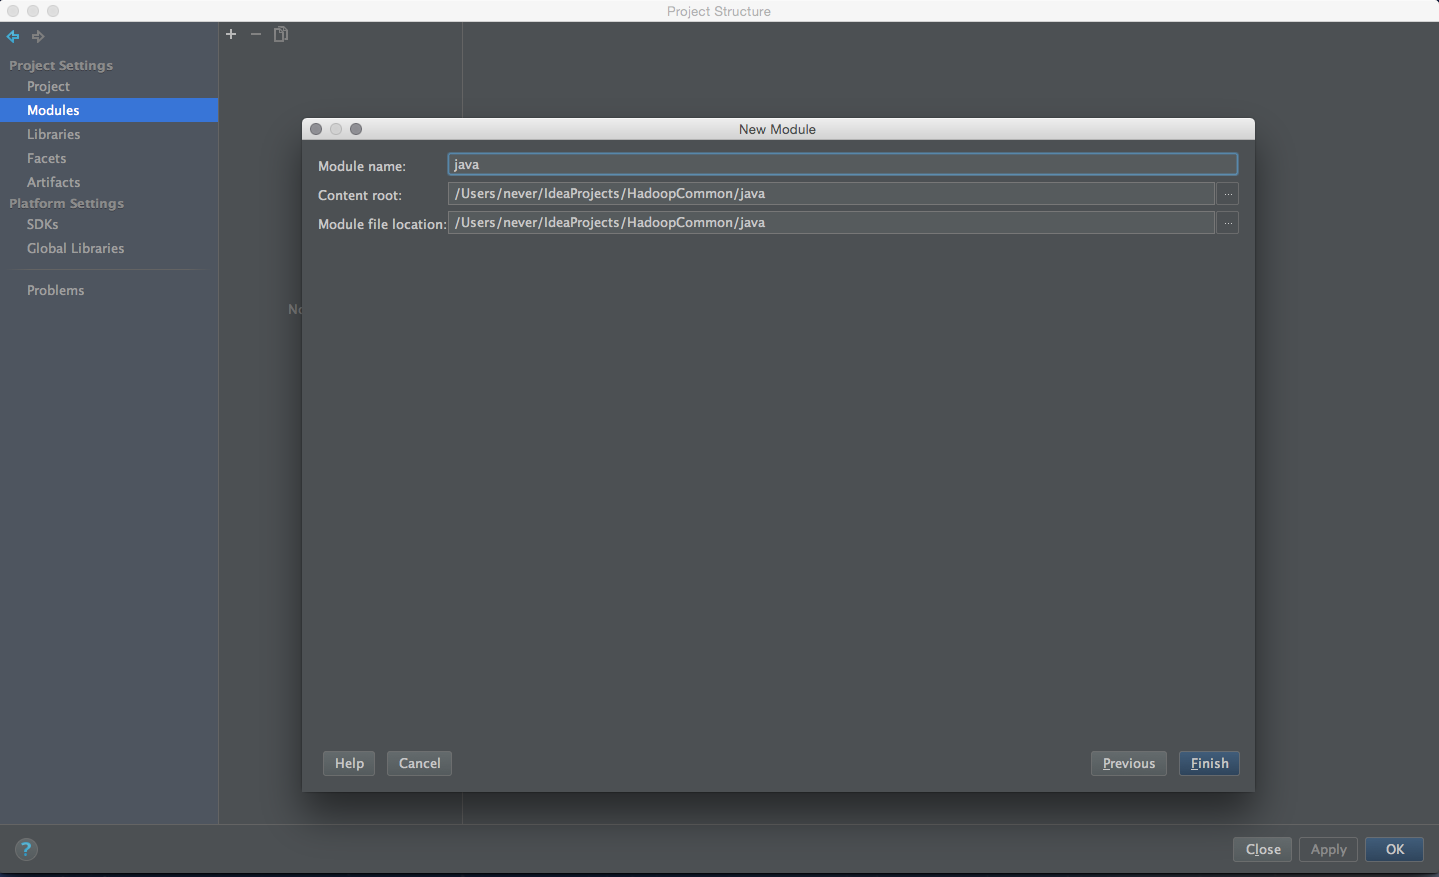
\includegraphics[width=\textwidth]{image/env/cr25.png}

然后将Hadoop-release-0.21.0的common中的代码以及core-default.xml和log4j.properties复制到工程目录java/src下,如下图所示

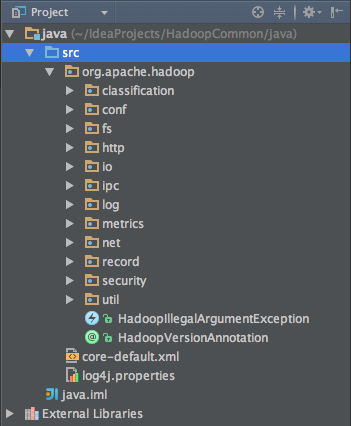
\includegraphics[width=\textwidth]{image/env/cr26.png}

然后将Hadoop依赖的jar包复制到lib/中,这些依赖可以通过解析Ant的Build.xml获得,也可以通过提取Ant编译好的工程中的Build目录中的相关jar包来完成。

然后回到Project Structure配置页面,打开Modules -> Dependencies选项卡,可以看到如下界面

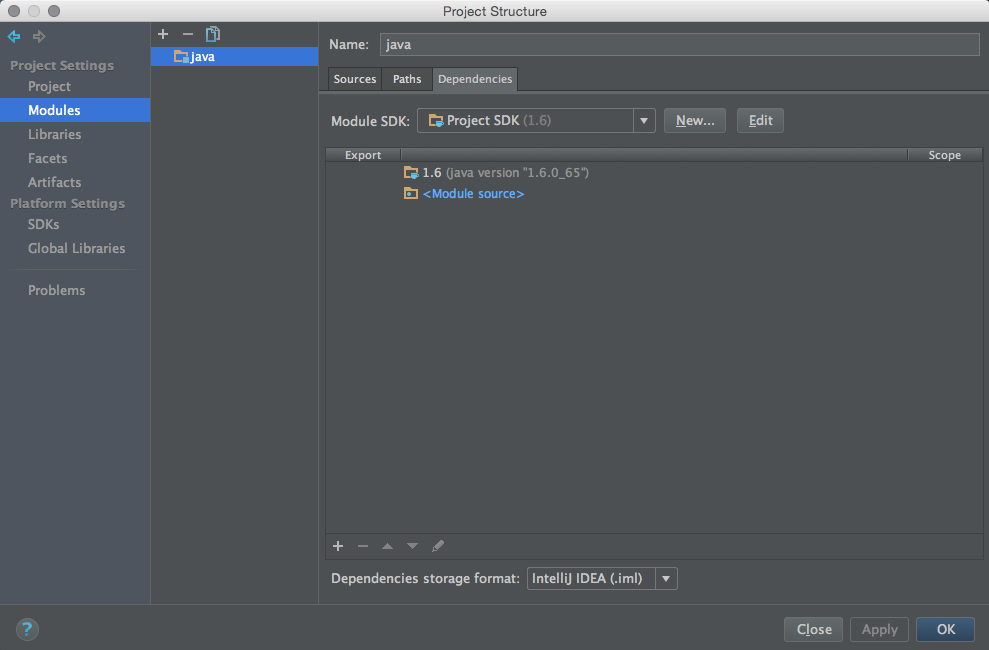
\includegraphics[width=\textwidth]{image/env/cr27.png}

点击添加JARs or Dictionarys

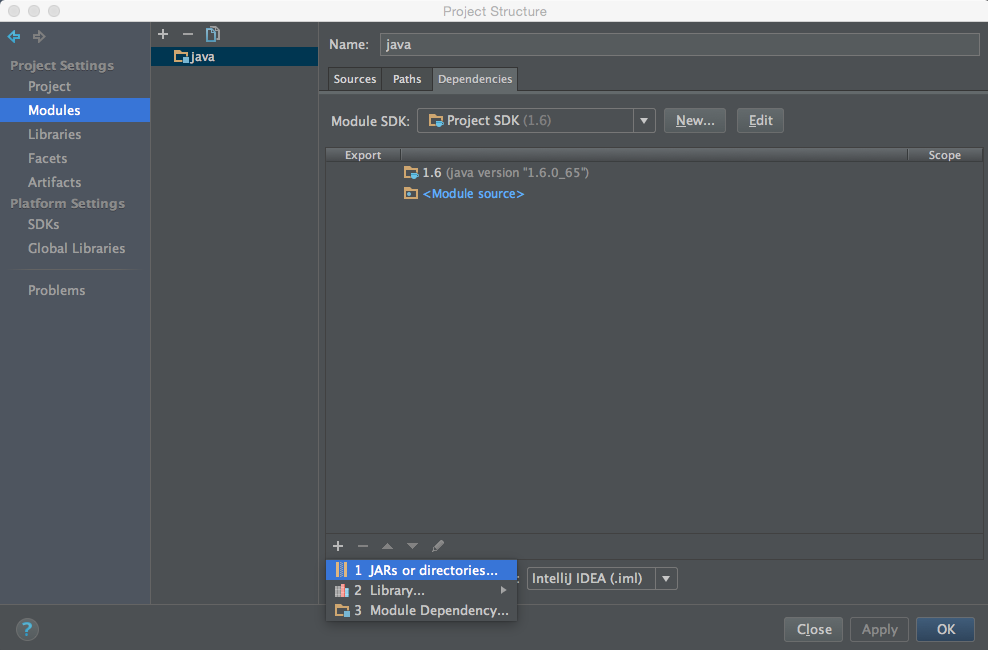
\includegraphics[width=\textwidth]{image/env/cr28.png}

选择刚才添加的java/lib/目录

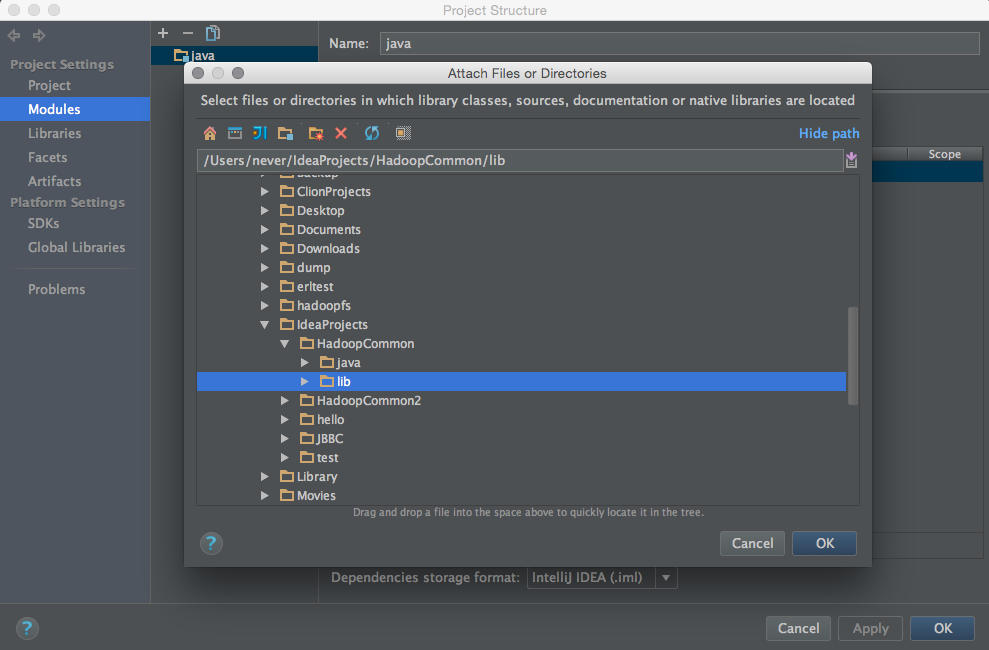
\includegraphics[width=\textwidth]{image/env/cr29.png}

然后配置运行参数,点击Run -> Edit Configuration,添加一个Application

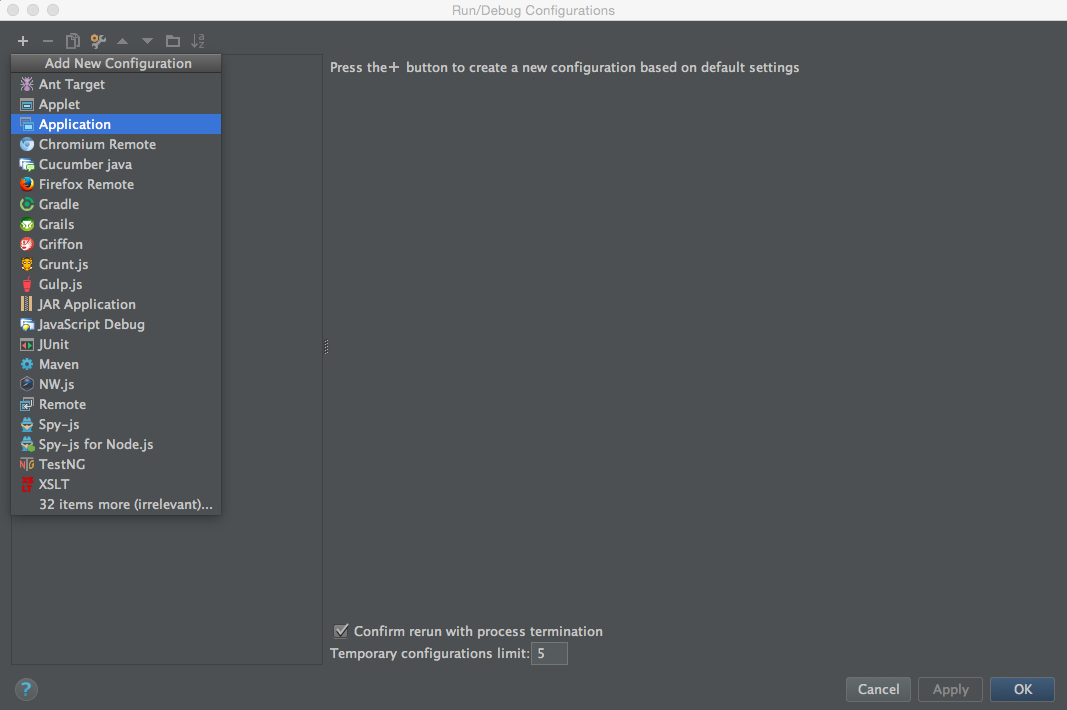
\includegraphics[width=\textwidth]{image/env/cr30.png}

添加好之后在里面输入相关的参数,主要是配置Main Class为org.apache.hadoop.fs.FsShell,在Program Arguments里输入要执行的命令行参数,如图所示

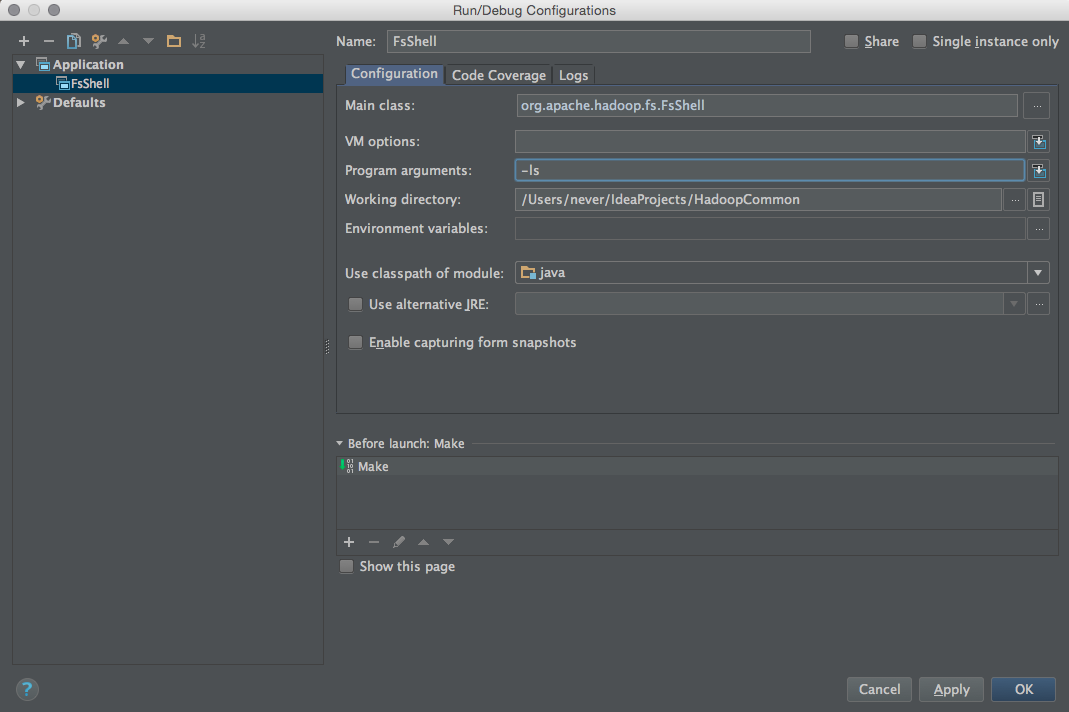
\includegraphics[width=\textwidth]{image/env/cr31.png}

好了,现在完成了基本的配置,可以运行程序了,点击Run,可以看到如下的运行结果

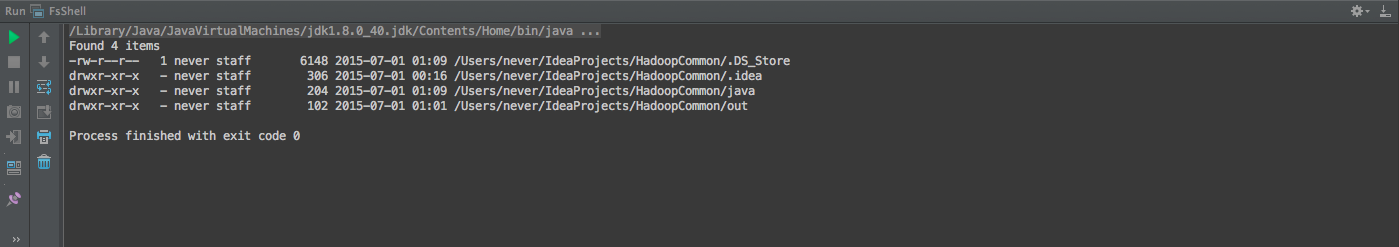
\includegraphics[width=\textwidth]{image/env/cr32.png}

那么现在可以在程序中添加断点,来观察程序的运行过程,函数的入口在org.apache.hadoop.fs.FsShell类中的main函数,添加断点之后,点击Run - > Debug来开始调试,可以看到程序开始位置的断点如下

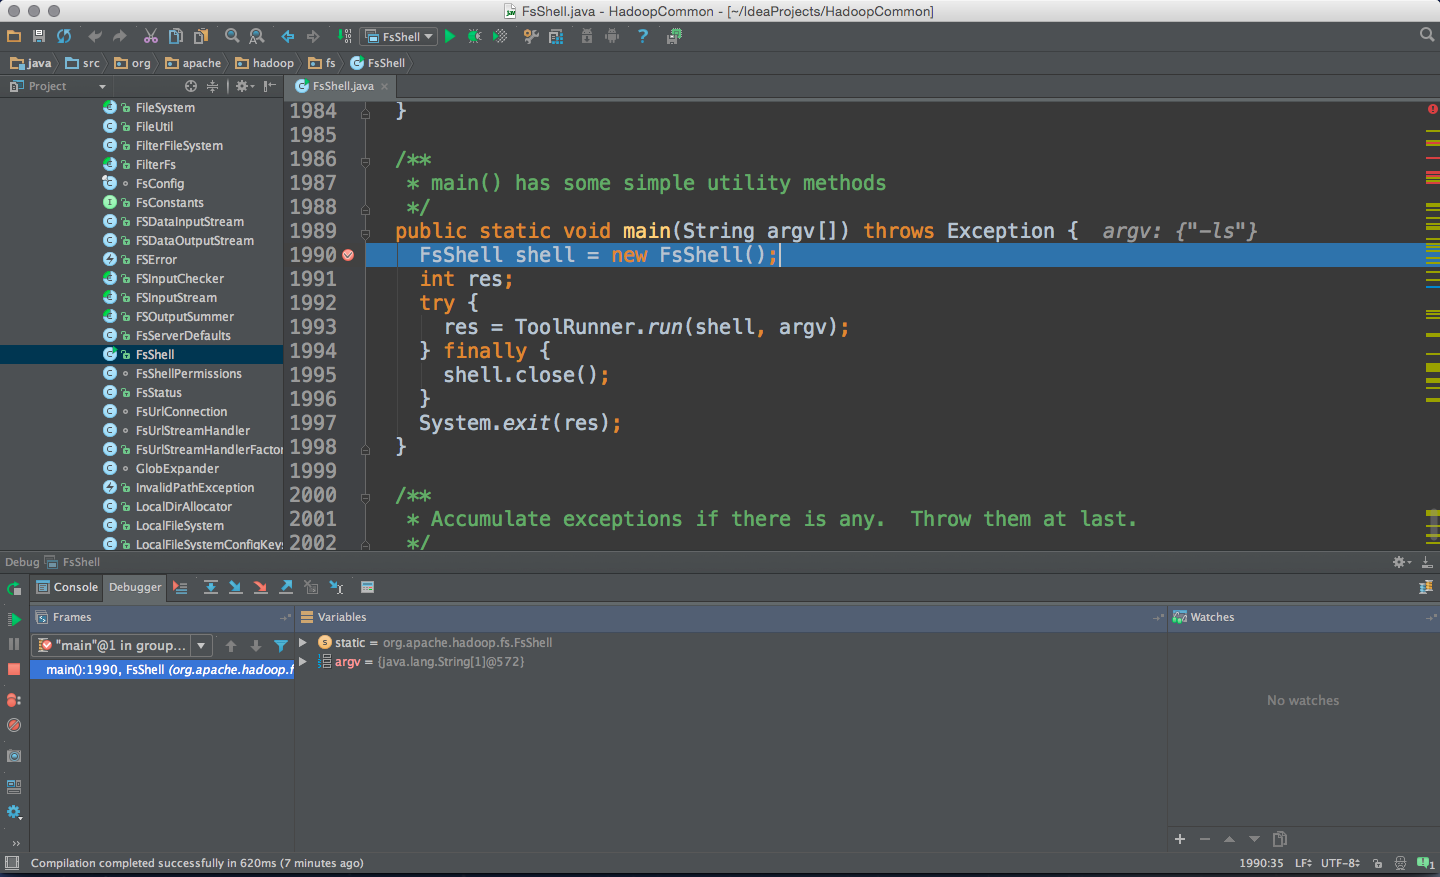
\includegraphics[width=\textwidth]{image/env/cr33.png}

根据对源码的阅读,可以发现,FsShell类实现了Tool接口,其运行过程主要交给另一个类--ToolRunner负责,这个工具类的主要作用是,解析程序传入的参数,加载程序设置,然后调用传入的Tool类的run方法,具体执行的方法如下所示

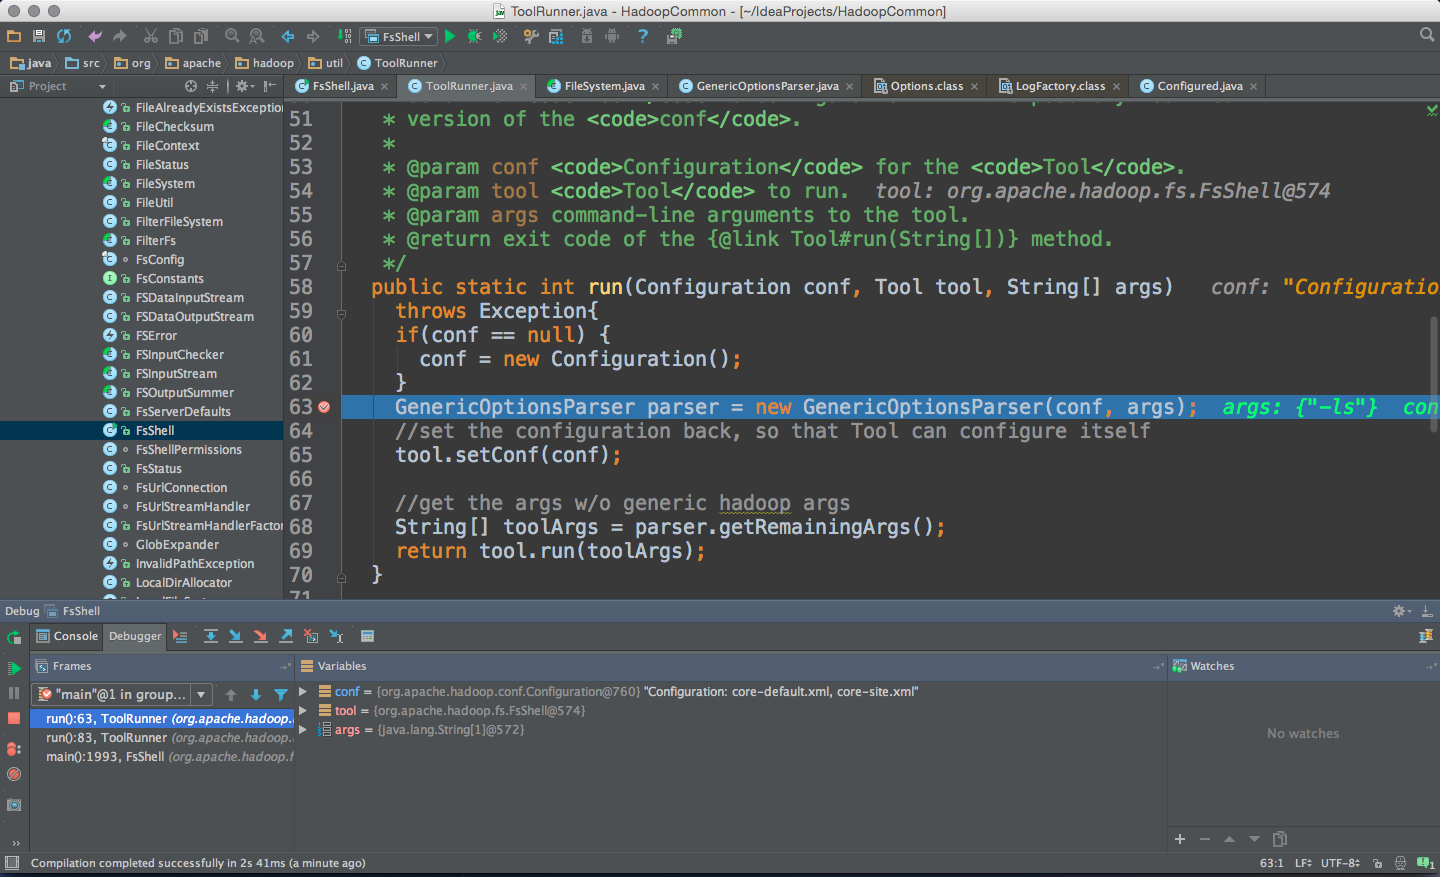
\includegraphics[width=\textwidth]{image/env/cr34.png}

现在进入FsShell的run方法,这个方法根据输入的命令行参数,如``-ls'',``-put''等,调用不同的函数来处理

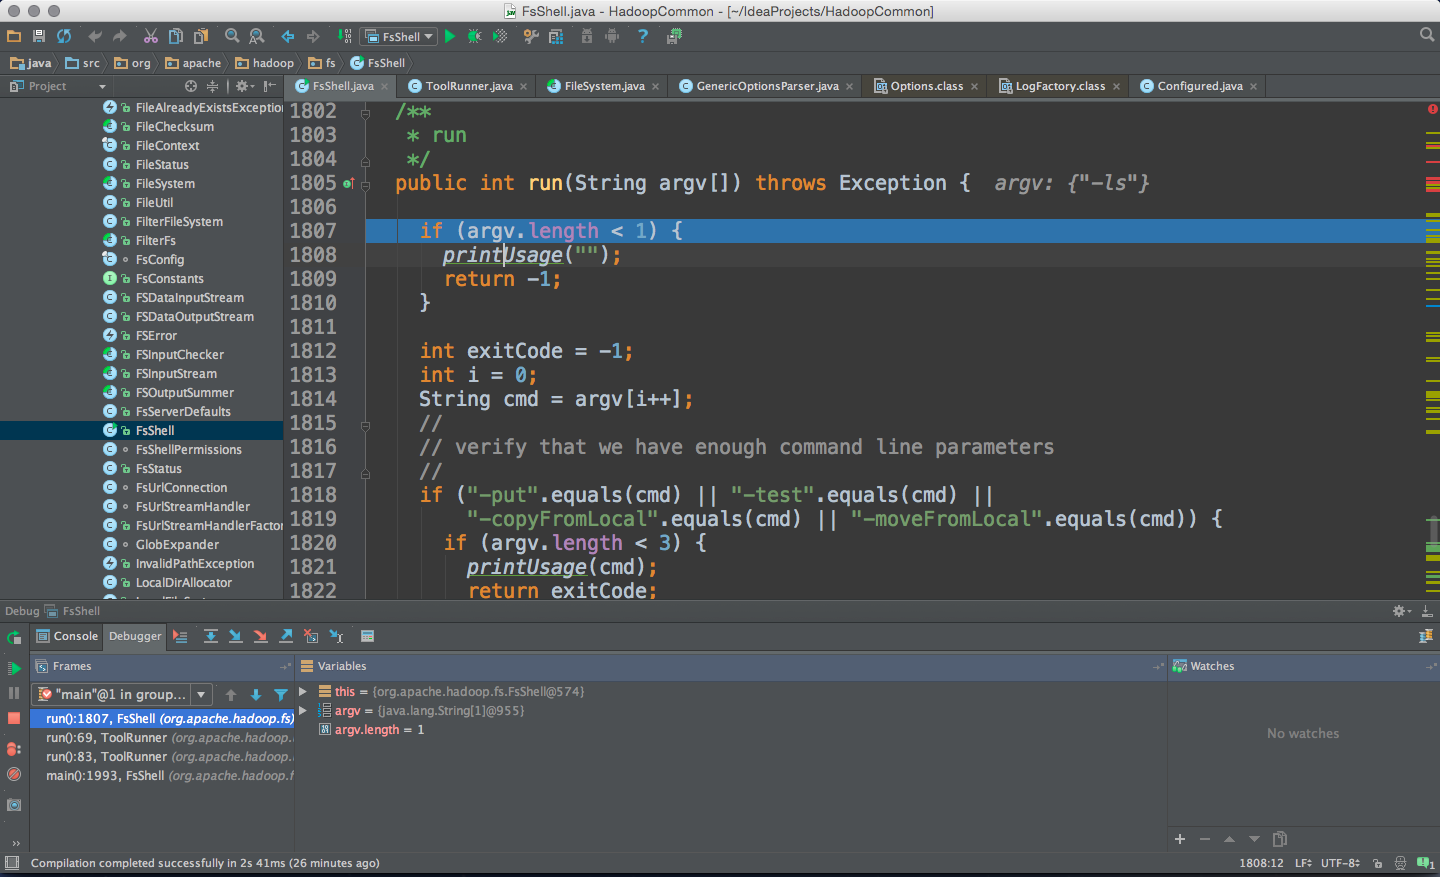
\includegraphics[width=\textwidth]{image/env/cr35.png}

当我们的输入参数为``-ls''时,run方法会执行到此处

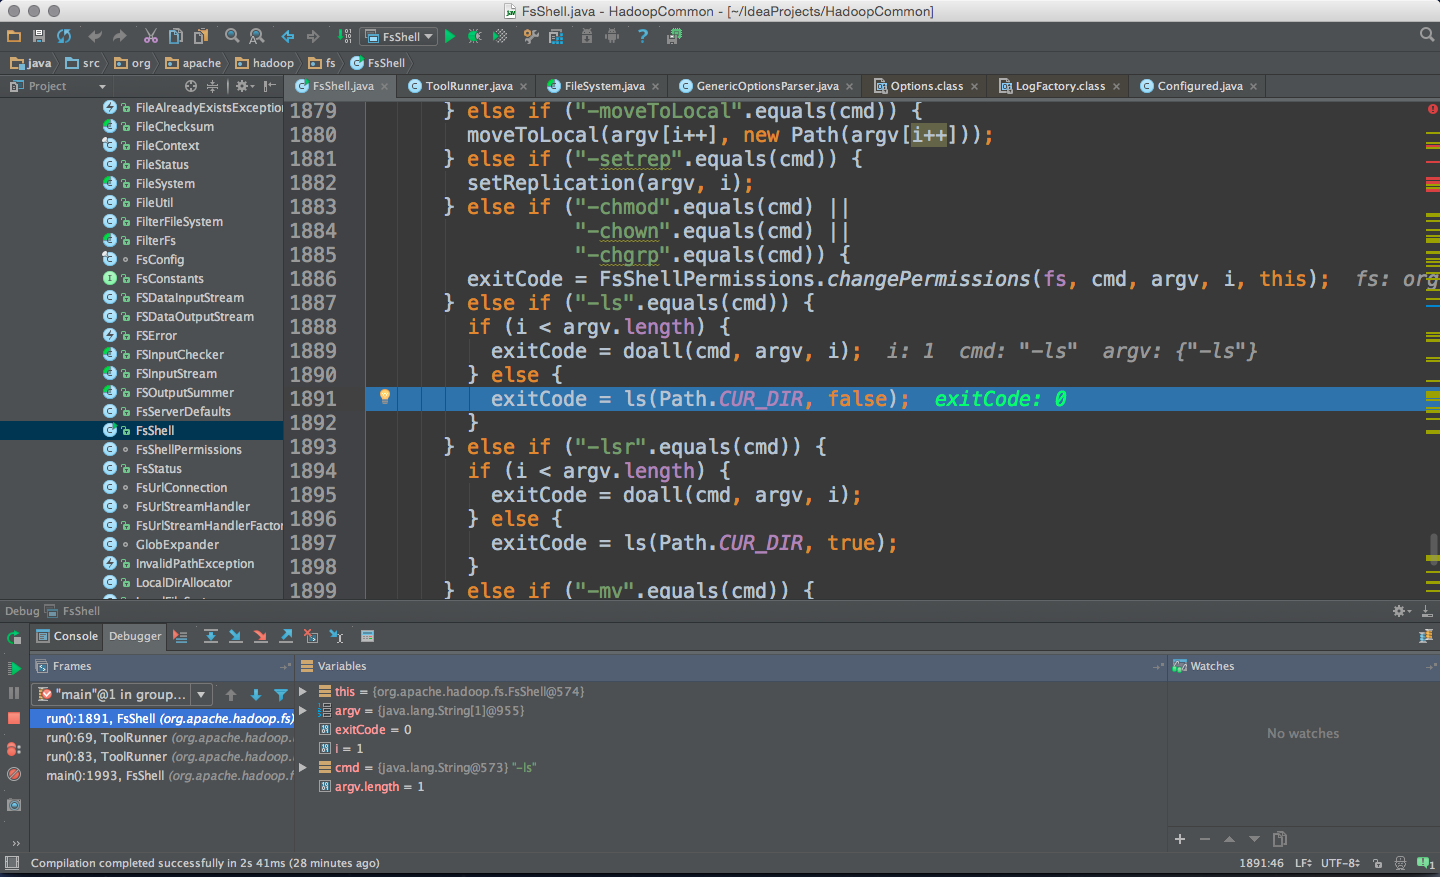
\includegraphics[width=\textwidth]{image/env/cr36.png}

可以看到我们没有提供第二个路径参数,这里默认就设置了Path为当前目录``''Path.CUR_ID'',即``''.''

接下来进入ls的具体执行步骤

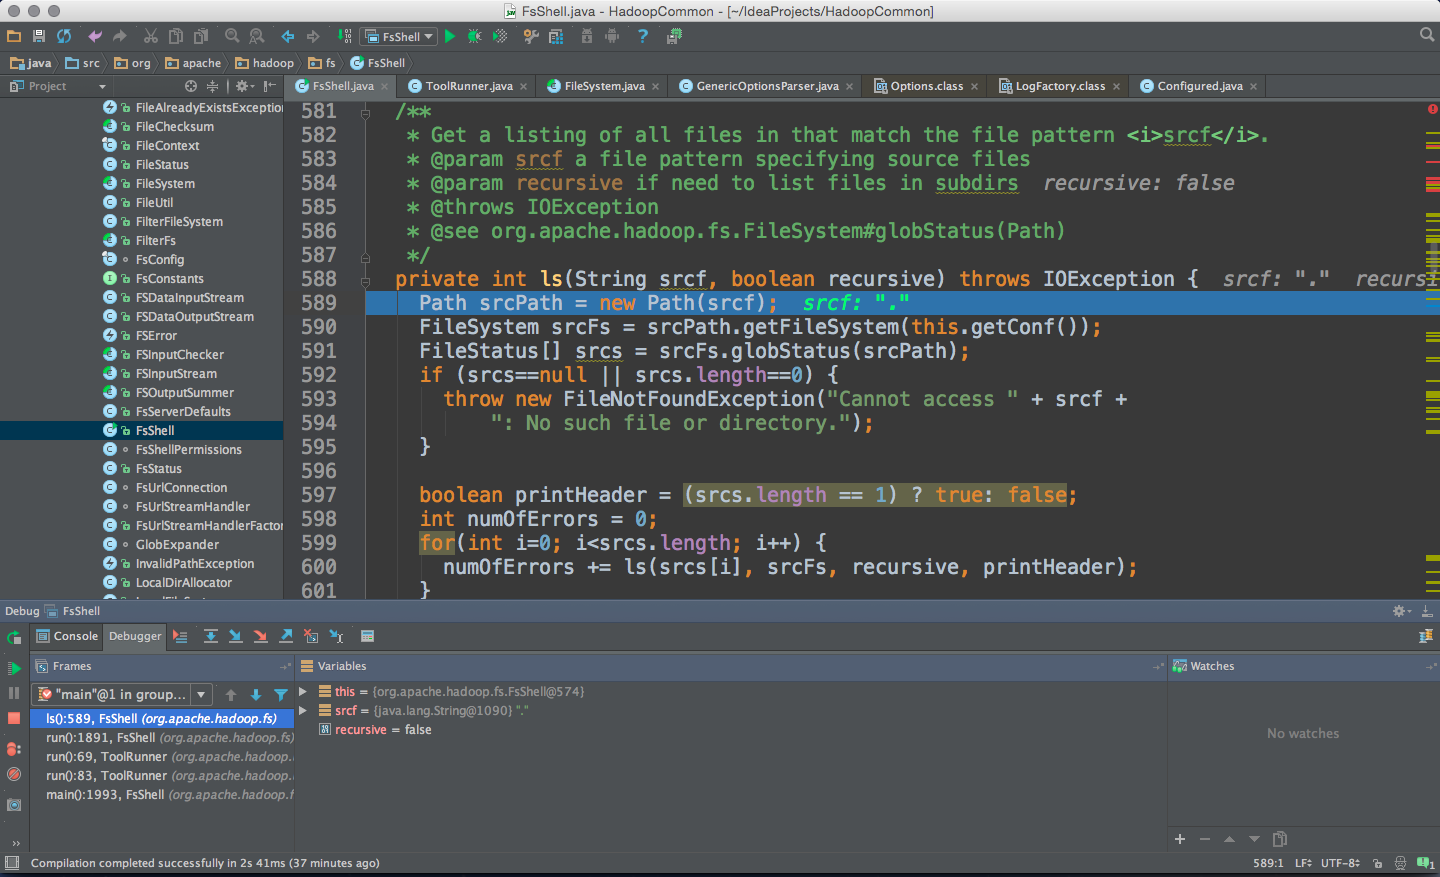
\includegraphics[width=\textwidth]{image/env/cr37.png}

首先,程序会用传入的path字符串构造一个Path对象,然后使用Path对象的getFileSystem方法,这个方法会接着调用FileSystem的静态方法get,首先在CACHE对象中寻找是否有已创建的对应文件系统,如果有就直接返回被cache的对象

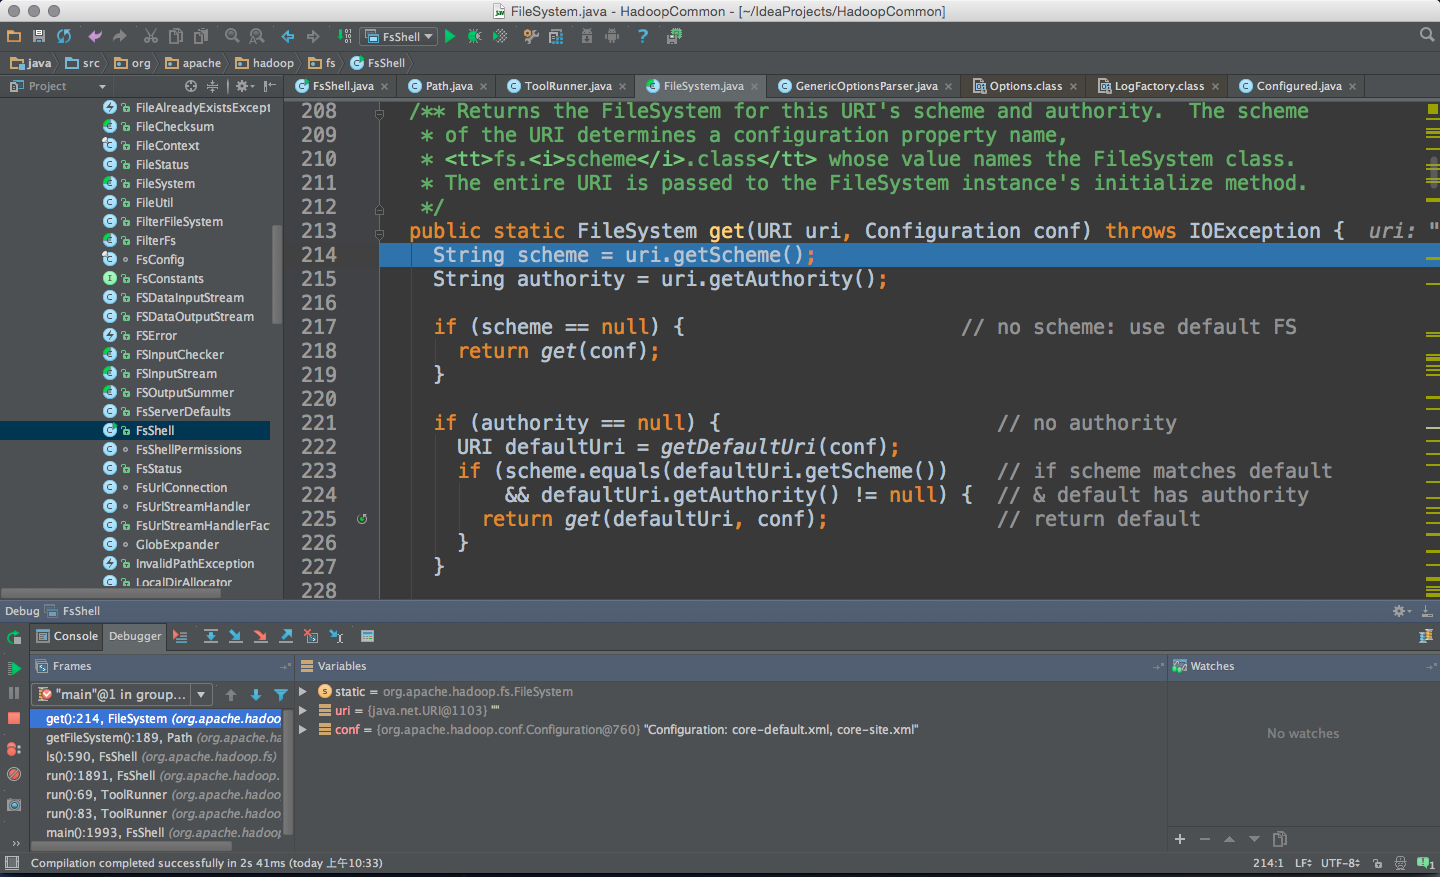
\includegraphics[width=\textwidth]{image/env/cr38.png}

如果CACHE中没有,则会最终调用FileSystem的createFileSystem,根据默认的配置文件,以及Path的uri中的Scheme来判断将要生成的具体的FileSystem对象

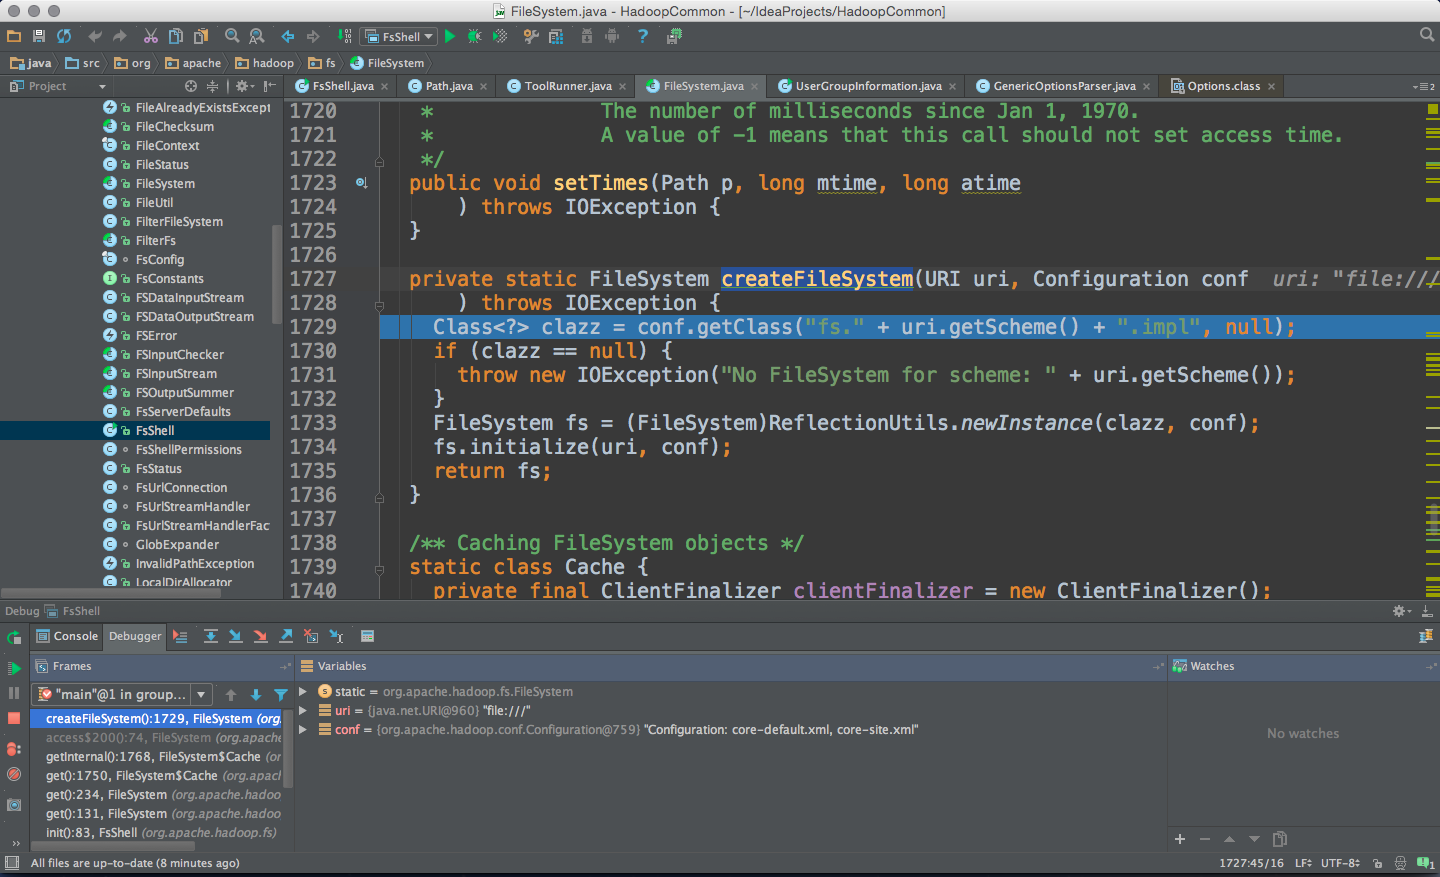
\includegraphics[width=\textwidth]{image/env/cr39.png}

然后回到ls函数执行过程,可以看到这里调用了生成的FileSystem对象的globStatus方法,此方法会返回匹配输入文件名的所有文件或文件夹的FileStatus对象,然后根据每个对象是文件或者文件夹,将结果打印到终端。

注意这里的srcFS是一个org.apache.hadoop.fs.LocalFileSystem对象

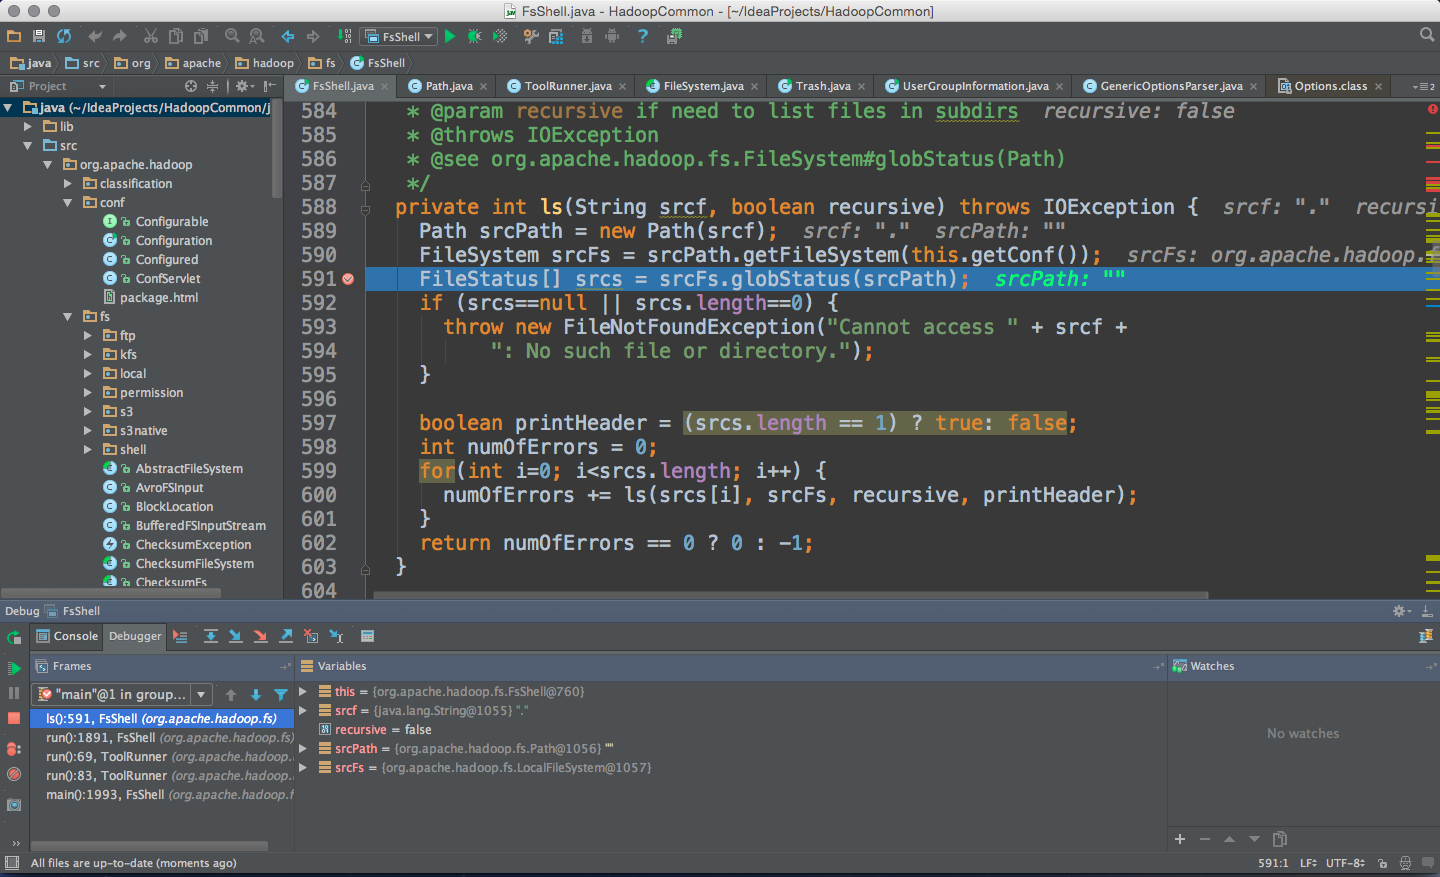
\includegraphics[width=\textwidth]{image/env/cr40.png}

接下来改变一下参数,现在将core-default.xml中的fs.defaultFS的值改为我们刚才设置的HDFS的namenode所在的位置

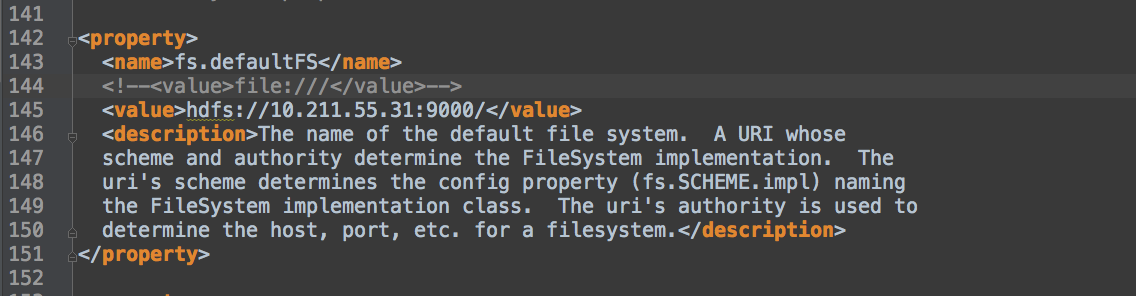
\includegraphics[width=\textwidth]{image/env/cr41.png}

现在重新进入调试

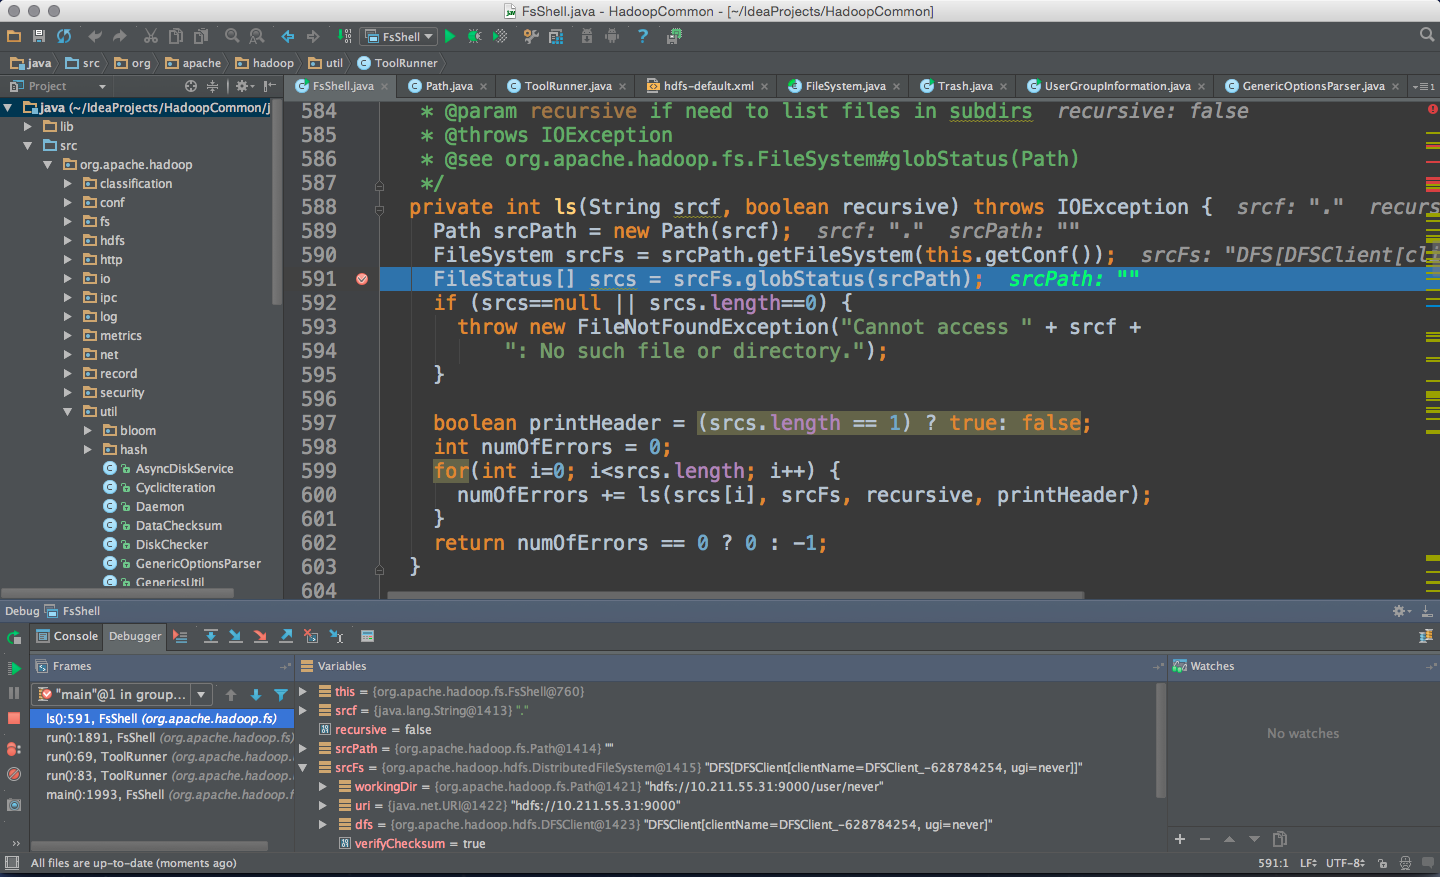
\includegraphics[width=\textwidth]{image/env/cr42.png}

可以看到现在生成的srcFS是一个org.apache.hadoop.hdfs.DistributedFileSystem对象,


以上内容说明,Hadoop文件系统的Shell入口在使用过程中,会通过读取配置文件,以及检测输入的uri的scheme,来定位所需要的继承了FileSystem类的具体类,然后通过调用这些具体类的方法来执行具体的功能
